%!TEX root = ../thesis.tex
% ******************************* Thesis Appendix C ********************************

\chapter{Reactor Building Edges}

\begin{figure}[htbp]
 \centering
 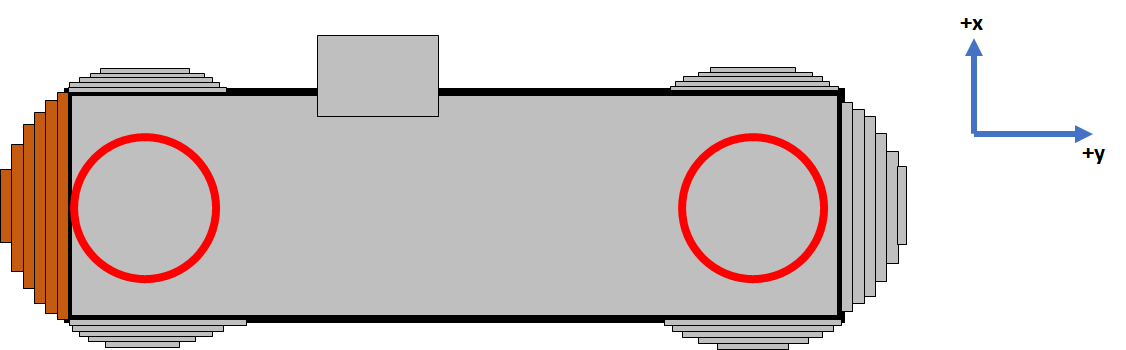
\includegraphics[width=\linewidth]{Chapter5/Figs/wylfaRasterNew/Slabs1.png}
 \captionof{figure}{Slabs for the left middle edge of the reactor building.} 
 \label{fig:slabs1}
\end{figure}

\begin{figure}[htbp]
 \centering
 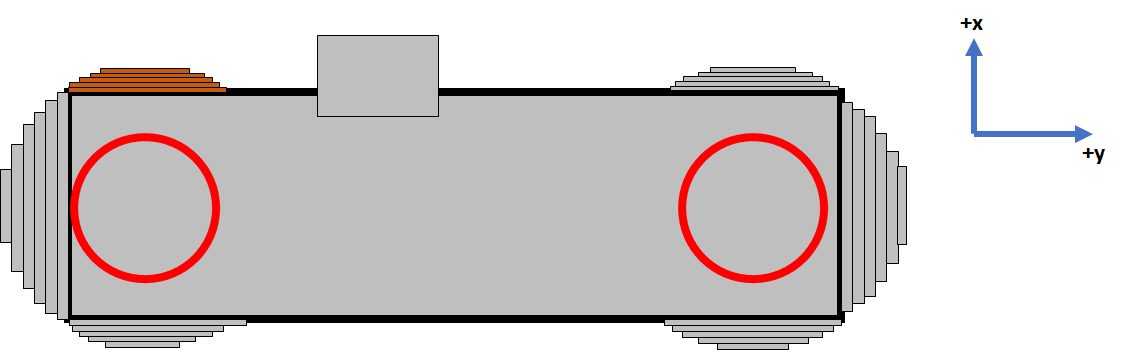
\includegraphics[width=\linewidth]{Chapter5/Figs/wylfaRasterNew/Slabs3.png}
 \captionof{figure}{Slabs for the left upper edge of the reactor building.} 
 \label{fig:slabs3}
\end{figure}

\begin{figure}[htbp]
 \centering
 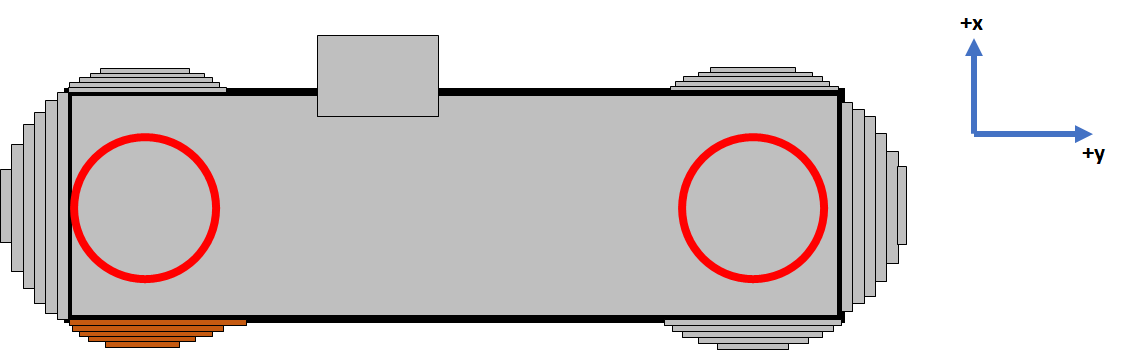
\includegraphics[width=\linewidth]{Chapter5/Figs/wylfaRasterNew/Slabs4.png}
 \captionof{figure}{Slabs for the left lower edge of the reactor building.} 
 \label{fig:slabs4}
\end{figure}

\begin{figure}[htbp]
 \centering
 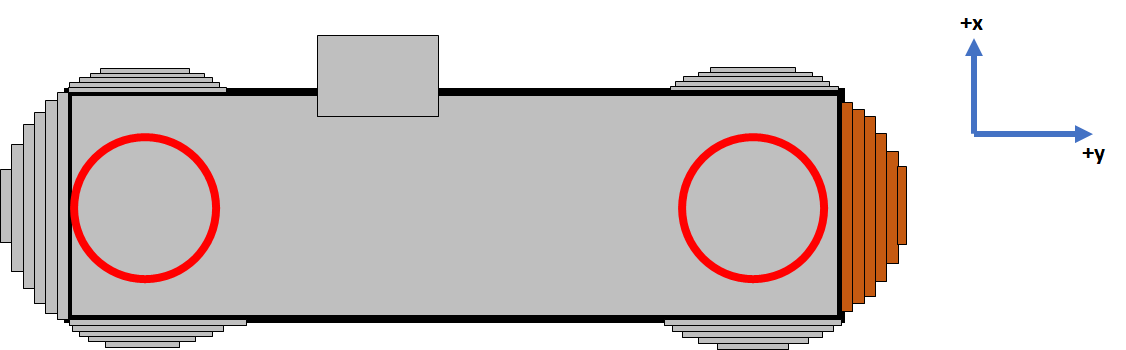
\includegraphics[width=\linewidth]{Chapter5/Figs/wylfaRasterNew/Slabs2.png}
 \captionof{figure}{Slabs for the right middle edge of the reactor building.} 
 \label{fig:slabs2}
\end{figure}

\begin{figure}[htbp]
 \centering
 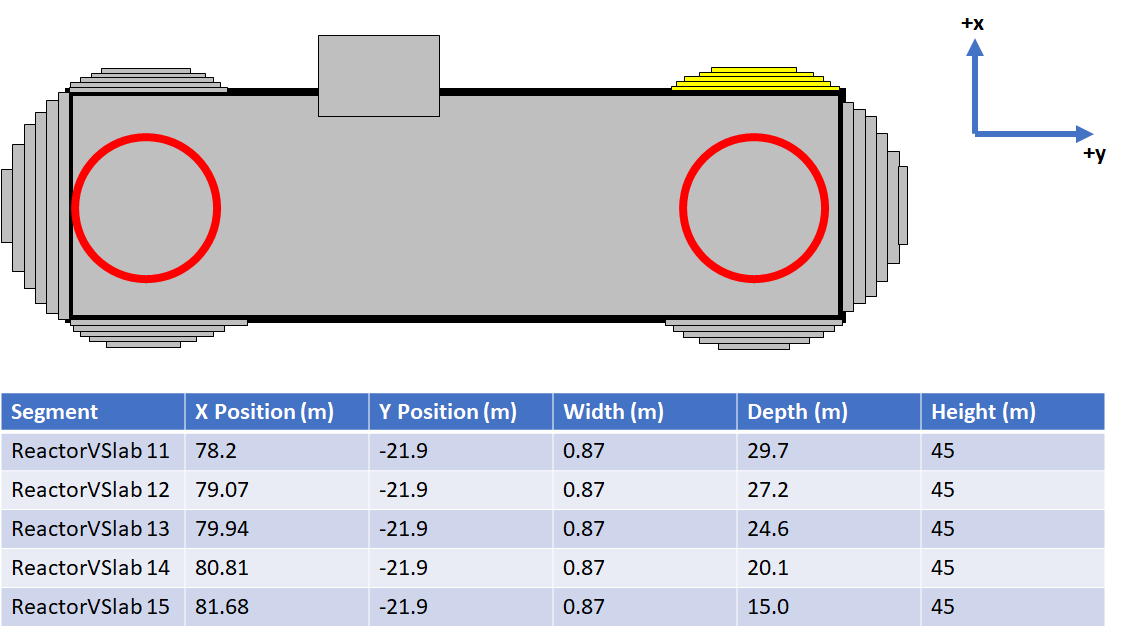
\includegraphics[width=\linewidth]{Chapter5/Figs/wylfaRasterNew/Slabs5.png}
 \captionof{figure}{Slabs for the right upper edge of the reactor building..} 
 \label{fig:slabs5}
\end{figure}

\begin{figure}[htbp]
 \centering
 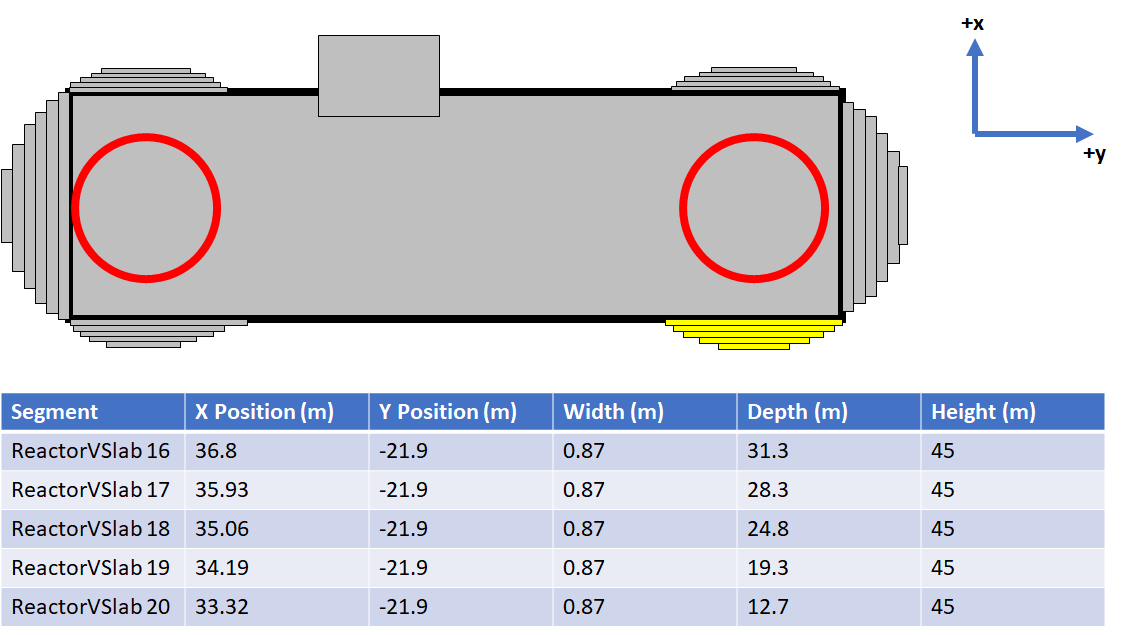
\includegraphics[width=\linewidth]{Chapter5/Figs/wylfaRasterNew/Slabs6.png}
 \captionof{figure}{Slabs for the right lower edge of the reactor building..} 
 \label{fig:slabs6}
\end{figure}